\documentclass[en]{../../../eplsummary}
\usepackage{framed}
\usepackage{placeins}
\usepackage{listings}
\usepackage{color}

\definecolor{dkgreen}{rgb}{0,0.6,0}
\definecolor{gray}{rgb}{0.5,0.5,0.5}
\definecolor{mauve}{rgb}{0.58,0,0.82}

\lstset{frame=tb,
  language=Java,
  aboveskip=3mm,
  belowskip=3mm,
  showstringspaces=false,
  columns=flexible,
  basicstyle={\small\ttfamily},
  numbers=none,
  numberstyle=\tiny\color{gray},
  keywordstyle=\color{blue},
  commentstyle=\color{dkgreen},
  stringstyle=\color{mauve},
  breaklines=true,
  breakatwhitespace=true,
  tabsize=3
}

\graphicspath{{res/}}

\hypertitle{algo-INGI2266}{7}{INGI}{2266}
{Houtain Nicolas}
{de Vogelaere Cyril}
{Pierre Schaus}

\section{Dynamic programing}

\subsection{Definition}

\textbf{Dynamic programming} is a method by recurrence in order to solve complex problem.
\begin{itemize}
    \item breaking it down into a collection of simpler subproblems
    \item solving each of those subproblems just once, and storing their solutions in memory
    \item[$\rightarrow$] Next time the same subproblem occurs, instead of 
recomputing its solution, only looks up to the previously computed solution.
Thereby \textbf{saving computation time at the expense of storage space}.
\end{itemize}

\subsection{Solving the knapsack problem with DP}

\subsubsection{The knapsack problem}
\begin{itemize}
    \item A set of item $I$
    \item for each item $i \in I$ is associated a value $v_i$ and a weight $w_i$.

    \item[Goals] 
        \begin{tabular}{m{3cm}m{12cm}}
            $\sum_{i \in I} v_i x_i$: & Maximize the value of selected items\\
            $\sum_{i \in I} w_i x_i \le C$ & Under constraint that the total
            capacity cannot exceed a given maximal capacity $C$ \\ 
            $x_i \in \{0,1\}$ & And an item cannot be partially selected \\
        \end{tabular}
\end{itemize}

Note that Knapsack is an NP-Complete problem as it can be used
to find a solution to the subset-sum problem, which is NP-complete.

\paragraph{Subset-sum problem}

Given a set of natural number and a capacity K. 
Find a subset S such that :
$$\sum_{i \in S} c_i = K$$


\subsubsection{Solutions}
\begin{itemize}
    \item \textbf{DP for knapsack in 0(Cn)}.

        Refer to the optimal objective of the problem with capacity $k$ and
        items \{1,…,j\} $\in$ I as $O(k,j)$. We can easily notice that :

        \begin{itemize}
            \item $O(k,0) = 0 \text{\footnotemark}$
            \item $ O(k,j) = \begin{cases} 
                    max(O(k,j-1) , vj +O(k-wj,j-1))\text{\footnotemark} & if \quad w_j \leq k \\
                    O(k,j-1) & otherwise
                \end{cases}$
        \end{itemize}
        \footnotetext{As their are no elements to choose from}
        \footnotetext{Bellman's equations}


        \begin{lstlisting}[caption=Knapsack DP]
val items = Array((1,1),(6,2),(18,5),(22,6),(28,7)) // (value,weight)
val C = 11
def O(j: Int, k: Int): Int = {
    if (j < 0) 0
    else {
        val (vj,wj) = items(j)
        if (wj > k) O(j-1,k)
        else O(j-1,k).max(vj + O(j-1,k-wj))
    }
}
println(O(items.size-1,C))
        \end{lstlisting}

        \begin{center}
    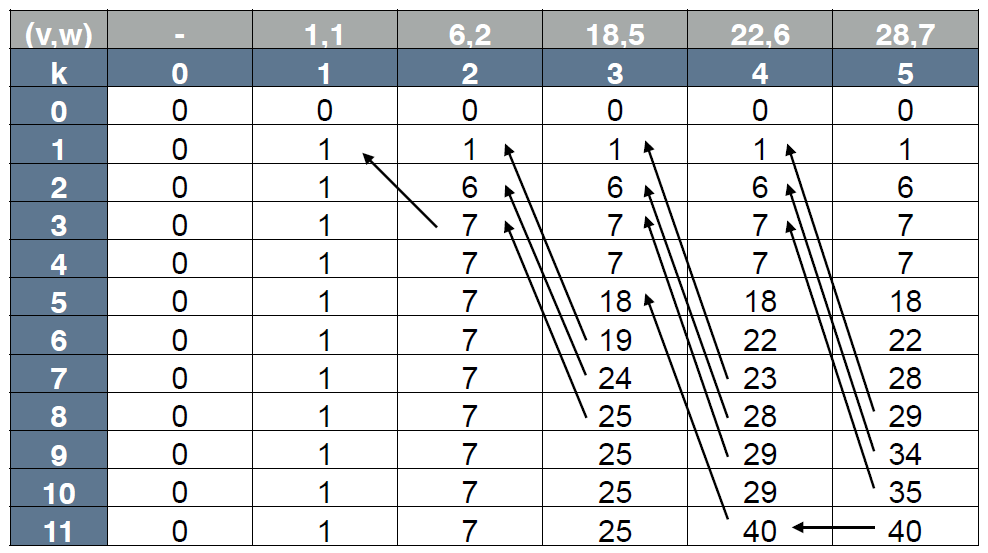
\includegraphics[width=7cm]{KnapsackDP.png}
        \end{center}

    \item \textbf{DP for knapsack in 0(Vn)}.

        Using a similar logic, it is also possible to define an algorithm which
        run in $\theta$(Vn) to compute knapsacks. Let $V = \sum_{i \in I} v_i$,
        we can redefine O(k,j) as O(w,j), the optimal weight using only items
        \{1,...,j\}. The equation will thus change as follow :

    \begin{itemize}
    \item $O(0,j) = O(w,0) = 0 \text{\footnotemark} $
    \item $ O(w,j) = \begin{cases}
                min(O(w,j-1), wi + O(w-v_j,j-1)) & if \quad v_j \leq p \\
                O(w,j-1) & otherwise
            \end{cases}$
        \end{itemize}
        \footnotetext{As $w_i > 0$ for all $i \in I$ and as we cannot have w > 0 with 
        an empty set.}
        \begin{center}
            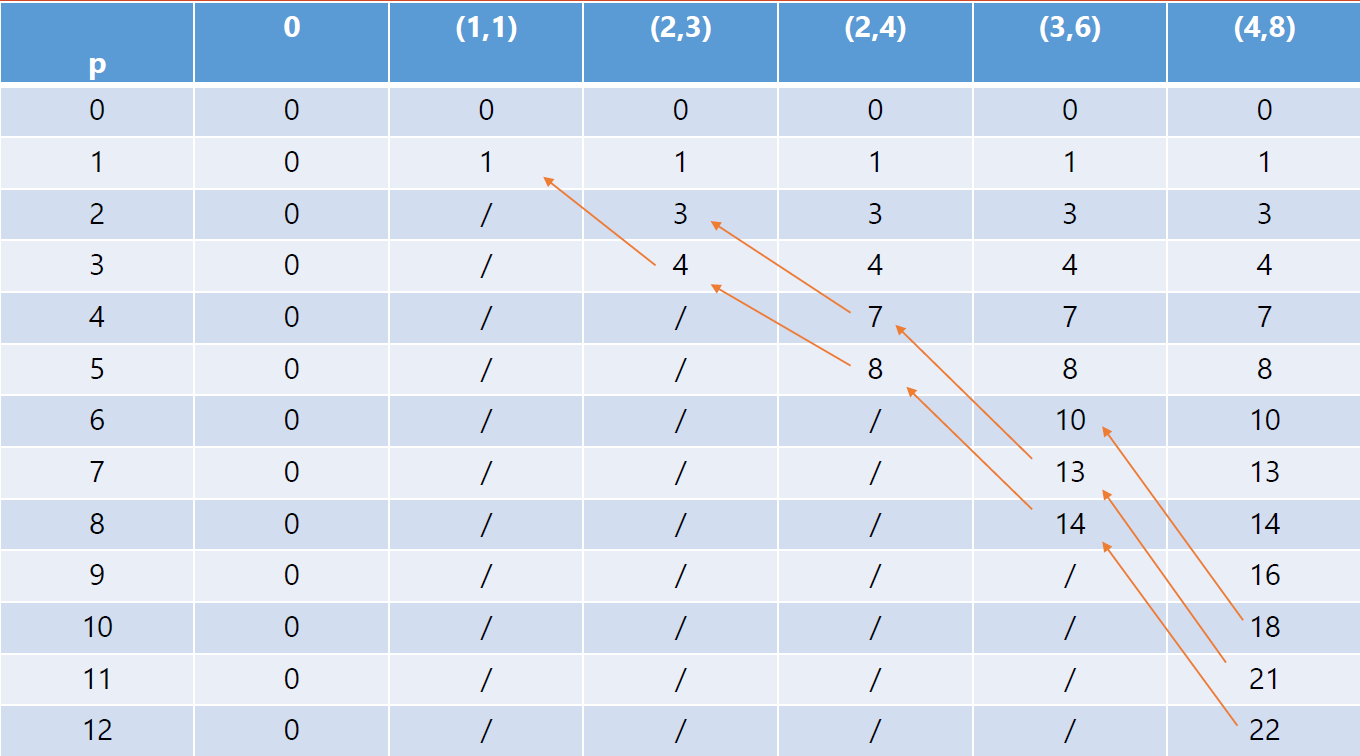
\includegraphics[width=7cm]{KnapsackDPAlgo2.png}
        \end{center}
\end{itemize}

\subsubsection{Cache usage}
\begin{tabular}{m{9cm}m{6cm}}
As explain, a cache is use in order to store computed value and avoid to recompute
it. In \textcolor{red}{red} we have the cells actually computed.
&
    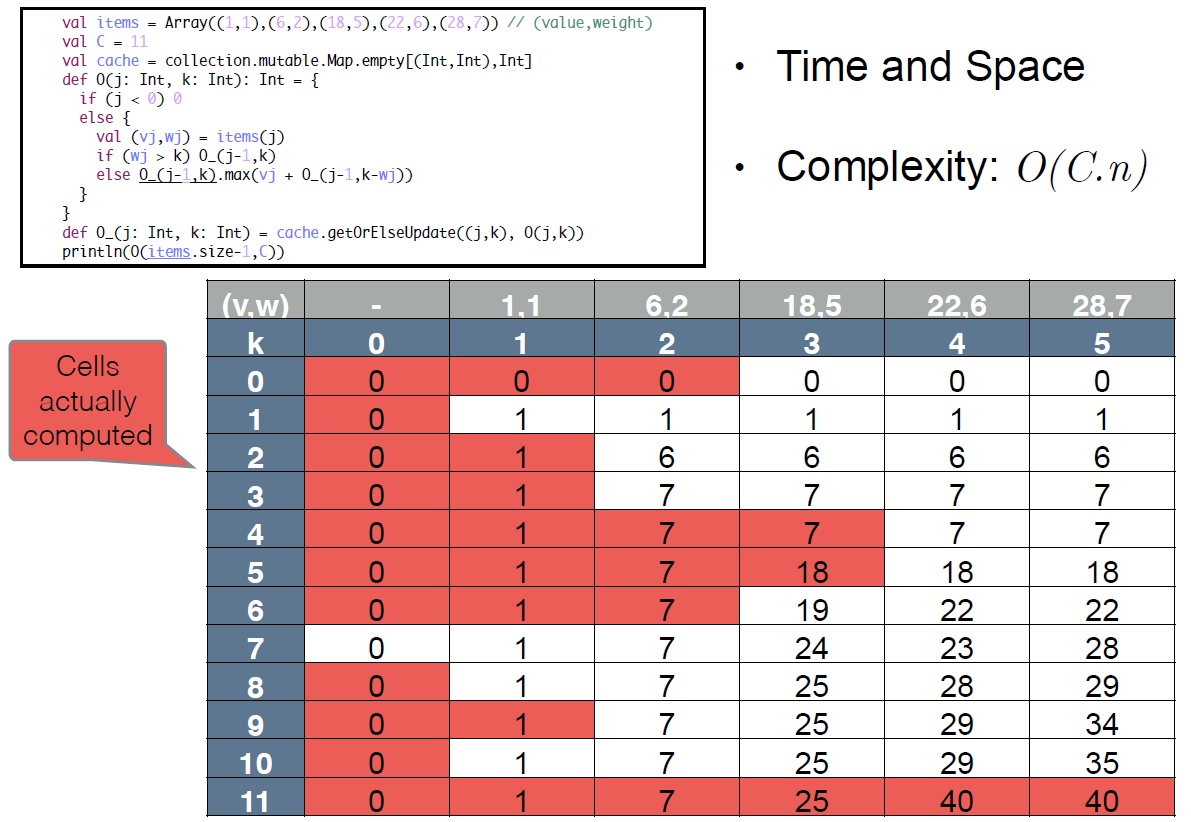
\includegraphics[width=6cm]{KnapsackDPAlgo1.png}
\end{tabular}


\subsubsection{Pseudo-polynomial}

DP is \textsc{pseudo-polynomial}, since it is exponential in the 
\textit{length of input} ($log(C)$) which is the number of bits required to
encode the input ($C$). The complexity is thus exponential relatively to the
input size. This algorithm is \textbf{weakly NP-Complete} or
\textbf{pseudo-polynomial}\footnote{a numeric algorithm runs in
pseudo-polynomial time if its running time is polynomial in the numeric value
of the input, but is exponential in the length of the input – the number of
bits required to represent it.} as it is roughly polynomial for small values of
C while computing larger value is much more expensive\footnote{Not all
    NP-Complete algorithm are pseudo polynomial ! Like the traveling salesman
problem (TSP), for example.}.


\subsection{Other examples of DP algorithms}

Before reading this section, please remember that all algorithm that can be
implemented via dynamic programming are not ipso-facto pseudo polynomial ! Any
algorithm can be expressed with dynamic programming as long as it can be separated in
sub problems.

\subsubsection{Edit distance}


TODO

\subsubsection{TSP}
 
TODO



\subsection{Exam}
I give you a problem (for instance the TSP, Knapsack)
\begin{itemize}
    \item  Design a greedy algorithm
    \item  Design a Dynamic Programming formulation
    \item  Design a relaxation and upper/lower bound
        procedure and embed it in a Branch and Bound
    \item  Justify advantages and disadvantages of each
    \item  Apply the three techniques to a small instance
        manually
\end{itemize}



\section{Branch and bound}

\subsection{Definition}

A \textbf{branch-and-bound} algorithm consists of a systematic enumeration of candidate solutions by means of state space search: the set of candidate solutions is thought of as forming a rooted tree with the full set at the root. The algorithm explores branches of this tree, which represent subsets of the solution set. Before enumerating the candidate solutions of a branch, the branch is checked against upper and lower estimated bounds on the optimal solution, and is discarded if it cannot produce a better solution than the best one found so far by the algorithm.

\subsection{Solving the knapsack problem with B\&B}

Given the following knapsack problem :

\begin{figure}[!ht]
    \centering
    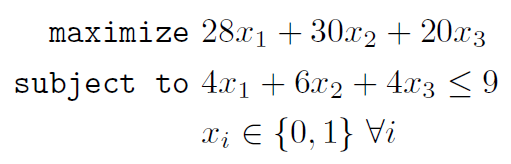
\includegraphics[width=0.4\linewidth]{KnapsackBBProblem.png}
    \label{fig:Knapsack_example}
\end{figure}
\FloatBarrier

We can choose to relax either of the constraint during the branch and bound procedure 
as to obtain a solution. The goal being to reduce the search space as much as possible
by calculating an upper bound as precise as possible.
Let us thus compare both options in the following sections.

\subsubsection{Capacity relaxation}

The first constraint that we can relax is the capacity constraint. The B\&B
calculation becomes fairly simple to implement as we only cut at tree branch when 
we have surpassed the capacity. The search space is thus reduced as such :

\begin{figure}[!ht]
    \centering
    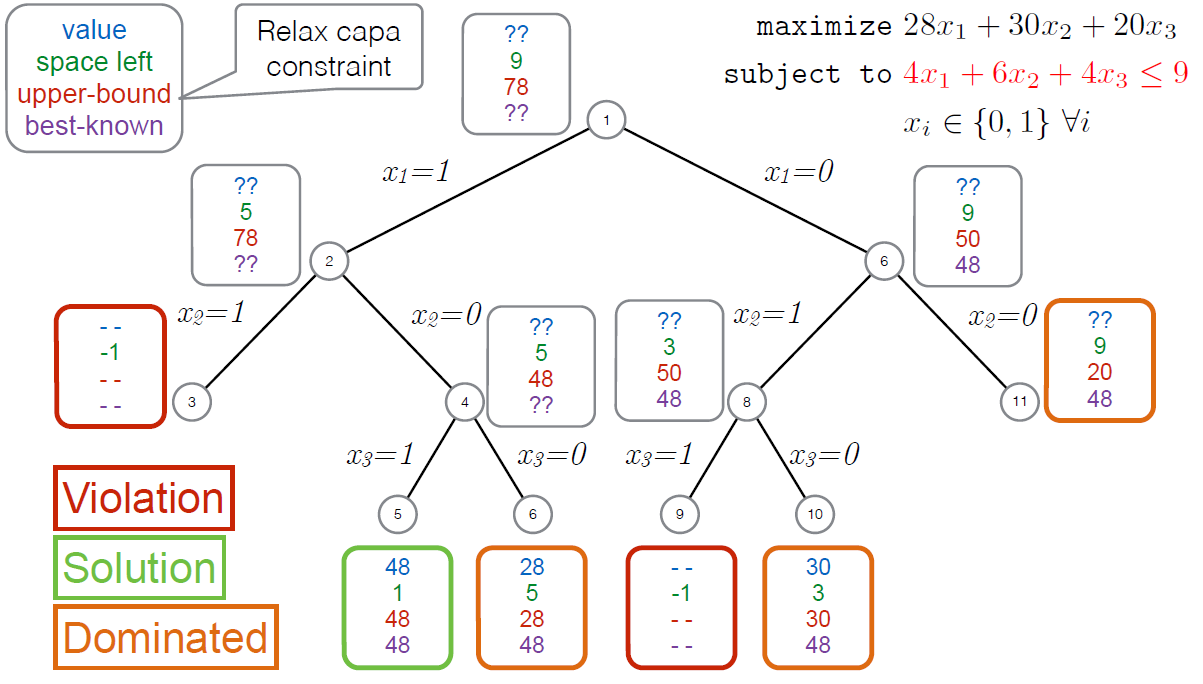
\includegraphics[width=\linewidth]{KnapsackBBCapaRelaxation.png}
    \label{fig:Knapsack_example}
\end{figure}
\FloatBarrier

Which, as you can see, is far from optimal as our upper bound are not close enough to their
real value.

\subsubsection{Linear relaxation}

This second relaxation is slightly harder to implement but yields better result, as 
the upper bound approximation is far better. Given a set sorted by ratio $v_i/w_i$,
the upper bound calculation procedure become as search for the first critical item j.
\newline

The first critical item j being the first item which cannot be fully added in our selection
due to capacity constraint. 

\begin{figure}[!ht]
    \centering
    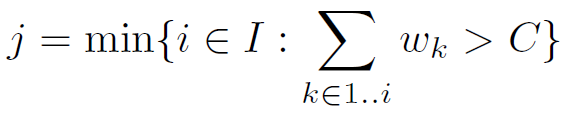
\includegraphics[width=0.4\linewidth]{KnapsackBBCriticalItem.png}
    \label{fig:Knapsack_example}
\end{figure}
\FloatBarrier

The upper bound can then be calculated as the sum of all item i < j plus as much of j
as we can squeeze in while respecting the capacity constraint.

\begin{figure}[!ht]
    \centering
    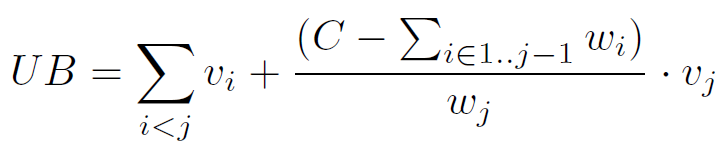
\includegraphics[width=0.5\linewidth]{KnapsackBBLinearRelaxationUB.png}
    \label{fig:Knapsack_example}
\end{figure}
\FloatBarrier

The search space is thus reduced as such :

\begin{figure}[!ht]
    \centering
    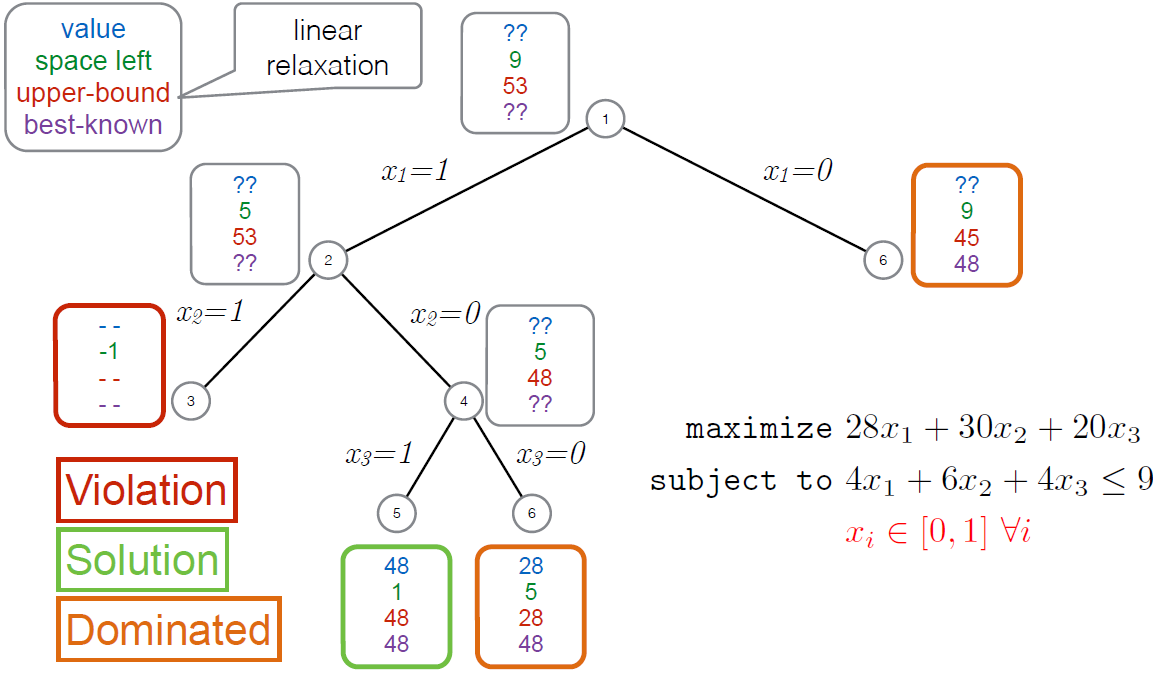
\includegraphics[width=\linewidth]{KnapsackBBLinearRelaxation.png}
    \label{fig:Knapsack_example}
\end{figure}
\FloatBarrier

As you can see, improving the precision of the upper-bound yields far better result. Take care however not to over/under estimate it (depending if you are on a maximisation or minimisation process) as it might prevent you to find the optimal solution.





\section{Search}
%TODO slides 2


\section{Linear programming}
\subsection{Definition}

Linear programming consist of a maximisation of a linear fonction subject to linear constraints.

\subsubsection{Example}

\begin{tabular}{m{8cm}m{5cm}}
    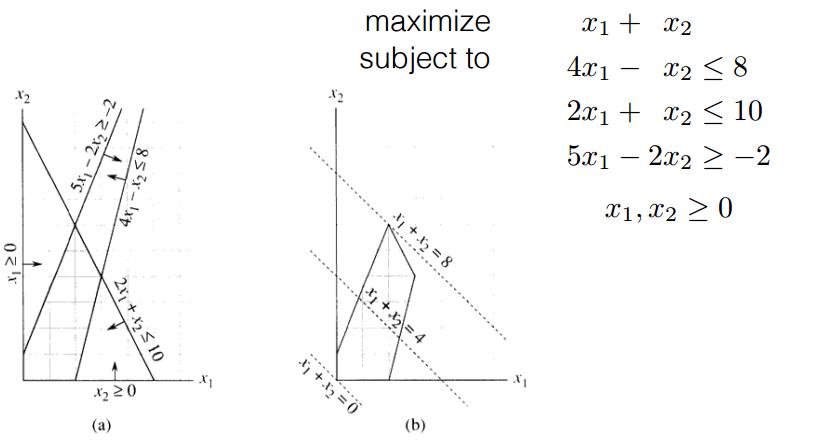
\includegraphics[width=7cm]{example1.png}
    &
    \begin{eqnarray*}
        \textrm{maximize } & x_1 + x_2 \\
        \textrm{subject to } & 4x_1 - x_2 & \leq 8 \\
                             & 2x_1 + x_2 & \leq 10 \\
                             & 5x_1 - 2x_2 & \geq -2\\
                            & x_1, x_2 \geq 0
        \end{eqnarray*}
\end{tabular}

\subsection{Polytope}

The solution space is a \textbf{polytope}. In a polytope, every point is a convex
combination of its vertices:
$$(\alpha x + (1 - \alpha)y) \in S \, \quad  with \quad \, \alpha \in
[0,1]$$

\begin{tabular}{m{8cm}m{4cm}}
    \begin{eqnarray*}
        \textrm{maximize } & c_1x_1 + ... + c_nx_n \\
        \textrm{subject to } & a_{11}x_1 + ... + a_{1n}x_n \leq b_1 \\
                             & ... \\
                             & a_{m1}x_1 + ... + a_{mn}x_n \leq b_m \\
        \end{eqnarray*}
        &
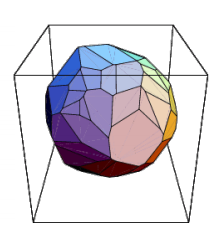
\includegraphics[width=3cm]{polytope.png}
\end{tabular}


\subsubsection{Theorem}
At least one of the points where the objective value is maximal is a vertex of the polytope.
\paragraph{Proof} : 
\begin{itemize}
    \item The maximum $x^{*}$ as a combination of the vertices of the
        polytope $v_{1},...,v_{t}$)
        $$x^{*} = \lambda_{1} v_{1} + ... + \lambda_{t} v_{t}$$

    \item Objective value at optimality can be expressed as a scalar
        product with $c$ a vector
        and the objective value at optimality can be expressed as a scalar product (c is a vector)
        $$c x^{*} = \lambda_{1} * (cv_{1}) + ... + \lambda_{t} * (cv_{t})$$
\end{itemize}

Let's assume that the maximum is not a vertex (each vertex is less good than $x^{*}$) \\
$$cx^{*} > cv_{i} \quad \forall i : 1 \leq i \leq t$$
Then we have 
\begin{align*}
cx^{*} =& \, \lambda_{1} * (cv_{1}) + ... + \lambda_{t} * (cv_{t}) \\
<& \, \lambda_{1} * (cx^{*}) + ... + \lambda_{t} * (cx^{*}) \\
<& \, (\lambda_{1} + ... + \lambda_{t}) (cx^{*}) \\
<& \, cx^{*}
\end{align*}

$\Rightarrow $ With this contradiction we can see that the maximal
$x^{*}$ must be a vertex.

\subsubsection{Algorithm}
We know that the best solution is located on a vertex of the
polytope:
\begin{enumerate}

    \item A naive approach would be to enumerate every vertices and take
        the one with the larget value. But, the problem is that the
        number of vertice grow exponentially with the number of
        inequality. 

    \item A better approach is the simplex algorithm. The idea is to
        move from one vertex to another with an improving objective
        function. We know this to be optimal thanks to the convexity of
        the polytope.
\end{enumerate}

\subsection{Simplex Algorithm}

\subsubsection{Standard and slack forms}
In order to use the simplex algorithm we need 
\begin{enumerate}
    \item Transform our linear problem  to  a \textbf{standard form}
        \begin{enumerate} 
            \item Replace equality to inequality
            \item If variable $x_j$ has no non-negativity
                constraint replace
                each occurrence by $x_j - x_k$
        \end{enumerate}
\begin{scriptsize}
        \begin{tabular}{m{7cm}cm{7cm}}
            \begin{eqnarray*}
                \textrm{maximize } & 2x_1 - 3x_2\\
                \textrm{subject to } & x_1 + x_2 &= 7\\
                                     & x_1 - 2x_2 &\leq 4 \\
                                     & x_1 &\geq 0\\
            \end{eqnarray*}
            & $\Rightarrow$ &
            \begin{eqnarray*}
                \textrm{maximize } & 2x_1 - 3x_2 + 3x_3\\
                \textrm{subject to } & x_1 + x_2 - x_3 & \leq 7\\
                                     & -x_1 - x_2 + x_3 & \leq -7  \\
                                     & x_1 - 2x_2 + 2x_3 & \leqq 4 \\
                                     & x_1, x_2, x_3 & \geq 0\\
            \end{eqnarray*}
        \end{tabular}
\end{scriptsize}

    \item then transform standard form to a \textbf{slack form }.
        $\Rightarrow$  Introduction of basis variable in order to find a 
        \textbf{Basic Feasible Solution}

\begin{scriptsize}
        \begin{tabular}{m{7cm}cm{7cm}}
            \begin{eqnarray*}
                \textrm{maximize } & 2x_1 - 3x_2 + 3x_3\\
                \textrm{subject to } & x_1 + x_2 - x_3 & \leq 7\\
                                     & -x_1 - x_2 + x_3 & \leq -7  \\
                                     & x_1 - 2x_2 + 2x_3 & \leqq 4 \\
                                     & x_1, x_2, x_3 & \geq 0\\
            \end{eqnarray*}
            & $\Rightarrow$ &
            \begin{eqnarray*}
                \textrm{maximize } & & 2x_1 - 3x_2 + 3x_3\\
                \textrm{subject to } & x_4 =& 7 - x_1 - x_2 + x_3   \\
                                     & x_5 =&  -7 - x_1 - x_2 + x_3   \\
                                     & x_6 =&  4 - x_1 + 2x_2 - 2x_3   \\
                                     & &x_1, x_2, x_3, x_4, x_5, x_6  \geq 0\\
            \end{eqnarray*}
        \end{tabular}
\end{scriptsize}


        Slack form can be described by $(N, B, A, b, c, v)$ where

        \begin{scriptsize}
            \begin{tabular}{m{5cm}m{5cm}m{5cm}}

        \begin{itemize}
            \item $N = 
                \begin{pmatrix}
                    1 & 2 & 3
                \end{pmatrix} $
            \item $B = 
                \begin{pmatrix}
                    4 & 5 & 6
                \end{pmatrix} $
            \end{itemize}
            &

        \begin{itemize}
            \item $A = 
                \begin{pmatrix}
                    -1 & -1 & 1 \\
                    -1 & -1 & 1 \\
                    -1 & 2 & -2 
                \end{pmatrix} $
            \item $c = 
                \begin{pmatrix}
                    2 & -3 & 3
                \end{pmatrix} $
            \end{itemize}
            &
        \begin{itemize}
            \item $b =  
                \begin{pmatrix}
                    -1 & -1 & 1 \\
                    -1 & -1 & 1 \\
                    -1 & 2 & -2 
                \end{pmatrix} $
            \item $v = 0 $
            \end{itemize}
            \end{tabular}
        \end{scriptsize}
\end{enumerate}

\subsubsection{Basic Feasible Solution}
When our problem is represented as a slack we can find a BFS. 
\begin{itemize}
    \item If we can find easily a BFS:
        \begin{enumerate}
        \item We set every non basic variable to 0
        \item Then we get the value of our basis variable and 
            the objective set to 0. 
    \end{enumerate}

\item IF it's not so easy because some basics variables will be less
    than 0:
        \begin{enumerate}
        \item Put all the variables to the right such that you have
            $0 = constraints ...$
        \item Replace 0 in each constraint with a new variable
            and minimize their sum
        \item If we have a objective equal to 0, this a BFS

            Else the problem is not feasible
    \end{enumerate}

\item \textit{Basic Feasible Solution} = vertex of the standard form.

\end{itemize}

\subsubsection{Pivot}
Now the simplex algorithm will improve this BFS with the
\textbf{pivot}. 
\begin{itemize}
    \item We will increase our non
        basics variables ($x_1, x_2, x_3$) and decrease the basics one
        ($x_5, x_6, x_7$).
    \item[But] we can not decrease
        the basics ones less than 0. 
\end{itemize}

So for every non basics variables that we
will increase, we must check at what value we must stop in order to have
no basics variables under 0.

\paragraph{Example}:
\begin{scriptsize}
    \begin{enumerate}
        \item 
            \begin{tabular}{m{7cm}cm{6cm}}
                \begin{eqnarray*}
                    \textrm{maximize } & 3x_1 + x_2 + 2x_3\\
                    \textrm{subject to } &  x_4 = 30 - x_1 - x_2 - 3x_3 &
                    \textcolor{red}{x_1 \leq 30}\\
                    &  x_5 = 24 - 2x_1 - 2x_2 - 5x_3  &
                    \textcolor{red}{x_1 \leq 12} \\
                    &  x_6 = 36 - 4x_1 - x_2 - 2x_3  &
                    \textcolor{red}{x_1 \leq 9}  \\
                    & x_1, x_2, x_3, x_4, x_5, x_6  \geq 0\\
                    \\
                    \textrm{Substitute } & x_1 = 9 - \frac{x_2}{4} - \frac{x_3}{2} - \frac{X_6}{4}\\
                \end{eqnarray*} 
                & $\Rightarrow $ &
                \begin{eqnarray*}
                    \textrm{maximize } & &27 + \frac{x_2}{4} + \frac{x_3}{2} -
                    \frac{3x6}{6} \\
                    \textrm{subject to } & x_1 =&  9 + \frac{x_2}{4} + \frac{x_3}{2} -
                    \frac{3x_6}{6} \\ 
                    & x_4 =& 21 - \frac{x_2}{4} - \frac{x_3}{2} - \frac{x_6}{4} \\
                    & x_5 =& 6 - \frac{3x_2}{2} + 4x_3 + \frac{x_6}{2} \\
                    && x_1, x_2, x_3, x_4, x_5, x_6  \geq 0\\
                \end{eqnarray*} 
            \end{tabular}
        
                \vspace{-1.5cm}
            \begin{tabular}{m{7cm}cm{6cm}}
            \item \begin{tabular}{m{6cm}}
                    \begin{eqnarray*}
                    \textrm{Under constraint }& \textcolor{red}{x_3 \leq
                18 \quad x_3 \leq \frac{42}{5} \quad x_3 \leq \frac{3}{2}}\\
                    \textrm{Substitute } & x_3 = \frac{3}{2} - \frac{3x_2}{8} 
                    - \frac{x_5}{4} + \frac{X_6}{8}
                \end{eqnarray*}
                \end{tabular}

                \vspace{-1cm}
            \item \begin{tabular}{m{6cm}}
                \begin{eqnarray*}
                    \textrm{Under constraint }& \textcolor{red}{x_2 \leq
                132 \quad x_2 \leq 4 }\\
                    \textrm{Substitute } & x_3 = \frac{3}{2} - \frac{3x_2}{8} 
                    - \frac{x_5}{4} + \frac{X_6}{8}
                \end{eqnarray*}
                \end{tabular}
                & $\Rightarrow $  &
                \begin{eqnarray*}
                    \textrm{maximize } & &28 \textcolor{red}{-} \frac{x_3}{6} 
                    \textcolor{red}{-}\frac{x_5}{6} \textcolor{red}{-}
                    \frac{2x_6}{3} \\
                    \textrm{subject to } & x_1 =&  8 + \frac{x_3}{6} + \frac{x_5}{6} -
                    \frac{x_6}{3} \\ 
                    & x_2 =& 4 - \frac{8x_3}{3} - \frac{2x_5}{3} + \frac{x_6}{3} \\
                    & x_4 =& 18 + \frac{x_3}{2} + \frac{x_5}{2} \\
                    && x_1, x_2, x_3, x_4, x_5, x_6  \geq 0\\
                \end{eqnarray*} 
                \end{tabular}
    \end{enumerate}
\end{scriptsize}


\subsubsection{Cycling and degeneracy}

Sometimes an iteration will leaves the objective value unchanged
(degeneracy). This can lead to cycling leaving us the same slack form at
two different iterations. Those cycles can be avoided by breaking ties
choosing the variables with the smallest index for example (Brand's
rule). (Line 3 and 8 of the simplex algorithm).

\subsubsection{Limit of the simplex algorithm}

Most of the time the simplex algorithm performs very well. But it has
been shown that on some particular problem we get a worst case scenario
of exponential complexity. LP solving is not NP Hard, there exists other
algorithm of polynomial complexity (Ellipsoid, Interior points). Those
algorithms are not necessarily better than the simplex.

\subsection{Pseudo-code}
\begin{tiny}
\begin{tabular}{m{8cm}m{8cm}}
    \begin{lstlisting}[mathescape]
SIMPLEX(A, b, c):
    (N, B, A, b, c, b) = INITIALAZE-SIMPLEX(A, b, c)
    while some index $j \in N$ has $c_j > 0$ do
*       choose an index $e \in N$ for which $c_e > 0$
            for each index $i \in B$ do
                if $a_{ie} > 0$: $\Delta_i = b_i / a_{ie}$
                else $\Delta_i = \infty$
*           choose an index $l \in B$ that minimizes $\Delta_i$
            if $\Delta_i = \infty$: return 'undbounded'
            else (N, B, A, b, c, v) = PIVOT(N, B, A, b, c, v, l, e)

    for $i \in [1, n]$ do 
        if $i \in B$: $x_i* = b_i$
        else $x_i* = 0$

    return ($x_1*, x_2*,..., x_n*$)
    \end{lstlisting}
    &
    \begin{lstlisting}[mathescape]
PIVOT(N, B, A, b, c, v, l, e):
// Compute the coefficients of the equations for new basic variable $x_e$
    $\widehat{b_e} = b_l / a_{le}$
    for each $j \in N - \{e\}$ do
        $\widehat{a_{ej}} = a_{lj} / a_{le}$
    $\widehat{a_{el}} = l / a_{le}$

// Compute the coefficients of the remaining constraints
    for each $i \in B - \{l\}$ do
    $\widehat{b_{i}} = b_{i} - a_{ie}\widehat{b_e}$
        for each $j \in N - \{e\}$ do
            $\widehat{a_{ij}} = a_{ij} - a_{ie}\widehat{a_{ej}}$
        $\widehat{a_{il}} =  - a_{ie}\widehat{a_{el}}$

// Compute the objective
    $\widehat{v} = v + c_e\widehat{b_e}$
    for each $j \in N - \{e\}$ do
        $\widehat{c_j} = c_j - c_e\widehat{a_{ej}}$
    $\widehat{c_l} = - c_e\widehat{a_{el}}$

// Compute new sets of basic and nonbasic variables
    $\widehat{N} = N - \{e\} \cup \{l\}$
    $\widehat{B} = B - \{l\} \cup \{e\}$

    return ($\widehat{N}, \widehat{B}, \widehat{A}, \widehat{b},
    \widehat{c}, \widehat{v}$)
    \end{lstlisting}
\end{tabular}
\end{tiny}


\subsection{Integer Linear Programming (NP-Hard)}

\begin{tabular}{m{9cm}m{6cm}}
    \begin{eqnarray*}
        \textrm{maximize } & \sum_{j=1}^n c_jx_j \\
        \textrm{subject to } & \sum_{j=1}^n a_{ij}x_j \leq b_i \quad & for
        \quad i=1,2,...,m \\
        & x_j \in N \quad & for \quad i=1,2,...,m
        \end{eqnarray*}
    &
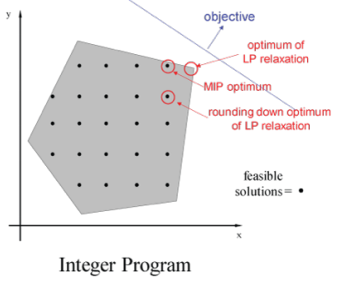
\includegraphics[width=6cm]{integerlinearprogram.png}
\end{tabular}


We can solve this using branch and bounds:

\begin{tabular}{m{12cm}m{6cm}}
    If at the optimal solution of
the linear programming relaxation, one variable is not an integer $x_i =
v$, we create two branches and adding those constraints will only
decrease the upper-bound.
    &
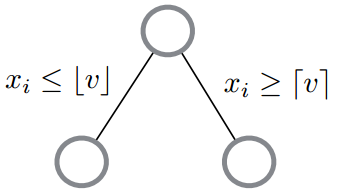
\includegraphics[width=3cm]{branch.png}
\end{tabular}



\subsection{Exam}
\begin{itemize}
    \item Formulate a linear program. 
    \item Be able to transform a LP into standard and slack form. 
    \item Explain and be able to find a initial BFS. 
    \item Apply the simplex algorithm on a small example. (be familiar with the pivoting)
    \item Explain how to detect an unbounded objective.

        $\Rightarrow$ You spot it when you have a var $x_i$ with a
        positive reduced cost in $z$ which always appears in constraints of the form 
        $b_i + x_i = x_n$
\end{itemize}



\section{Lagrangian relaxation}
\subsection{Definition}
The Lagrangian relaxation is a procedure that find a \textbf{lower
bounds}. This
lower bounds will allow to have better performances on the branch and
bounds of the problem starting with an initially good lower-bounds.

\begin{enumerate}
    \item We first relax the problem with the Lagrangian relaxation 
    \item We optimize the $\lambda$ with a sub-gradient algorithm 
    \item We get the optimal $\lambda$ and thus the optimal solution of
        the relaxed problem which is a good lower bounds.
\end{enumerate}

\subsection{Constrained Shortest Path Problem}
In order to represents the concepts discussed in this section, we will
need an example. Lets take the Constrained Shortest Path problem.

\begin{tabular}{m{8cm}m{6cm}}
    \begin{eqnarray*}
        \textrm{minimize } & \sum_{(i,j) \in A} c_{ij} \quad x_{ij} \\
        \textrm{subject to } & \textrm{flow conservation}\\
                            & \sum_{(i,j) \in A } \quad t_{ij} x_{ij} \leq T \\
                             & \forall (i, j) \in A, \quad x_{ij} \in \{0, 1\}
        \end{eqnarray*}

        \begin{itemize}
            \item A example can be to minimize distance with
                \textbf{time constraint} (NP-Hard problem).
        \end{itemize}
& 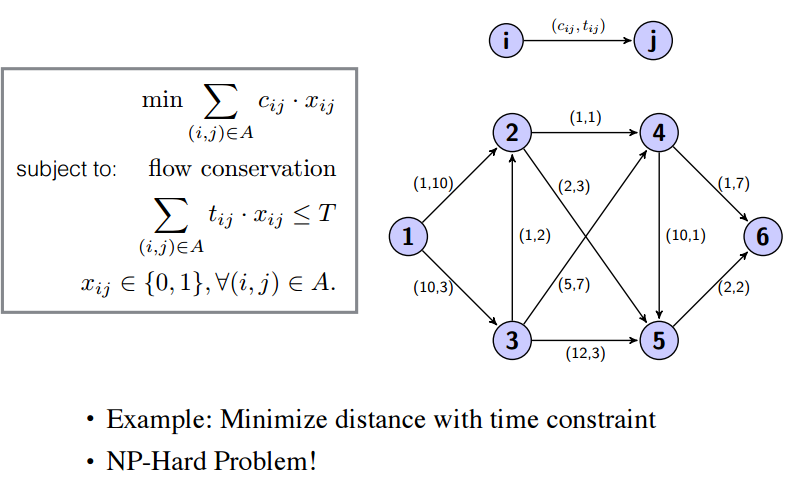
\includegraphics[width=7cm]{lagrangeexample.png}
\end{tabular}


\subsection{Relaxation}

If we remove the resource constraint, the problem is pretty easy. It is
a simple shortest path problem that can be easily resolved with
Dijkstra. What the Lagrangian relaxation does is \textbf{removing the
constraint} and \textbf{adding a new part} in our minimization part.

\begin{eqnarray*}
    L(\lambda) &=& min \sum_{(i,j)\in A} c_{ij} x_{ij} + 
    \textcolor{red}{\lambda \bigg(\sum_{(i,j)\in A} t_{ij} x_{ij} - T
    \bigg)} \\
    &=& min \sum_{(i,j)\in A} \Big(c_{ij} + \lambda t_{ij}\Big) x_{ij} - \lambda T\\
\end{eqnarray*}

$\Rightarrow$ We now have a simple shortest path problem 
where edges has a weight which is a
mixed value of time and distance for a given value of $\lambda$. 

\begin{itemize}
    \item Using this minimization with different $\lambda$ will return
        different solutions. 

    \item Some of them won't be feasibly and will violate the time
        constraint. If you are lucky one of the solution will be the
        optimal one. (hint: try $\lambda = 2$)
\end{itemize}

\subsection{Lagrangian dual}
Now our objective will be to find the best $\lambda$ in order to have
the best feasible solution (the best we can have with Lagrangian, not
necessarily the best of the actual problem, this algorithm is only used
to have a lower bound). We have our Lagrangian dual: 
$$L* = max_{\lambda} \Bigg( min \sum_{(i,j)\in A} (c_{ij} + x_{ij}) -
\lambda \big(\sum_{(i,j)\in A} (t_{ij} x_{ij}) - T\big) \Bigg)$$


\subsection{Find best $\lambda$}

\subsubsection{Brute force}
Formulate the minimization problem as a minimization over the set of all 
the feasible path $\rho \in P$:
$$L* = max_{\lambda} \Bigg( min \{ c_{p} + \lambda\big(t_p - T): \rho
    \in P \}\Bigg)$$

\subsubsection{Sub-gradient algorithm}

\begin{enumerate}
    \item Take an initial $\lambda$ and calculate the solution (Dijkstra resolution)
    \item We check if we are on a 
        \begin{itemize}
            \item increasing edge (violation of the constraint) 
            \item or a decreasing edge (constraint is respected). 
        \end{itemize}

        $\Rightarrow$ Depending of that we will respectively move to
        the right or to the left.
\end{enumerate}

\begin{tabular}{m{9cm}m{9cm}}
    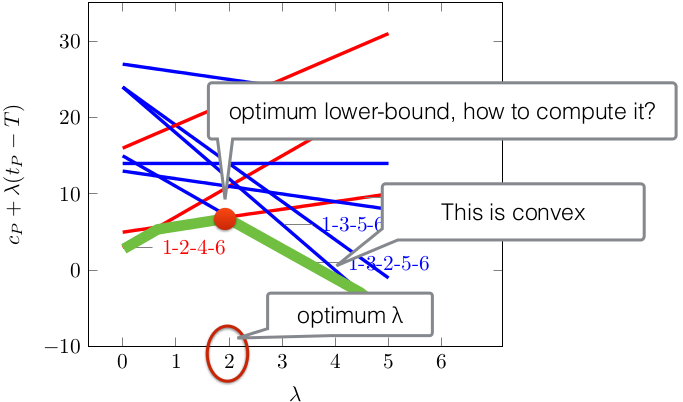
\includegraphics[width=9cm]{lag}
    &
    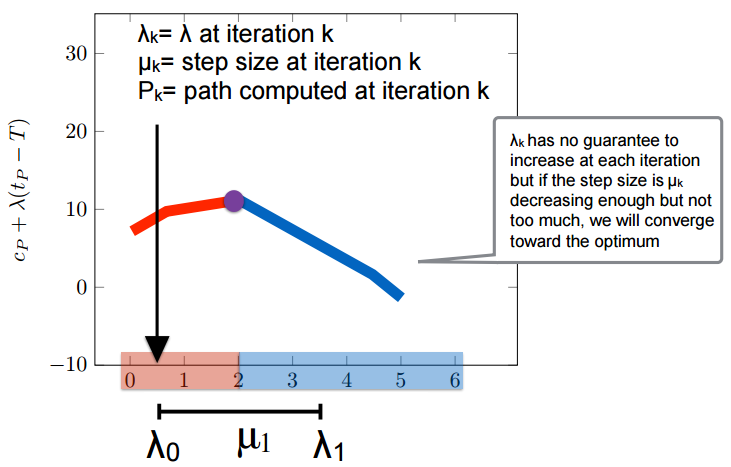
\includegraphics[width=7cm]{lagrangiangraph.png}
\end{tabular}


\begin{itemize}
    \item In order for the algorithm to converge we must reduce the size
        of the step at each iteration. 
    \item It is guaranteed to converge if $\mu_{k} \rightarrow 0$ and
        $\sum^{k}_{j=1} \mu_{k} \rightarrow \infty$.
    \item On the other hand the Lagrangian lower bounds has no
        guaranteed to increase at each step.
    \end{itemize}

\paragraph{Pseudo-code}:

\centerline{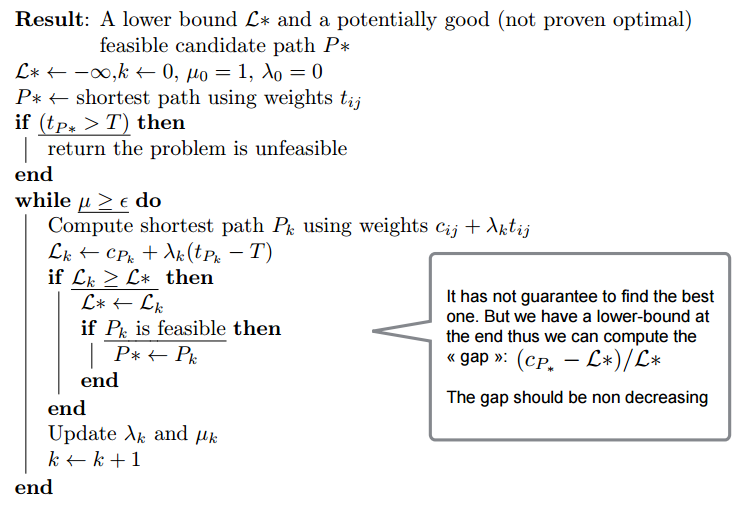
\includegraphics[scale=0.7]{lagrangepseudocode.png}}

\paragraph{Performances}

The Lagrangian relaxation is as good as the linear relaxation. But the
advantage of the Lagrangian one is that it will return feasible solution
during the process.

Typically the lower bounds will evolve along a curve that converge after x steps.

\centerline{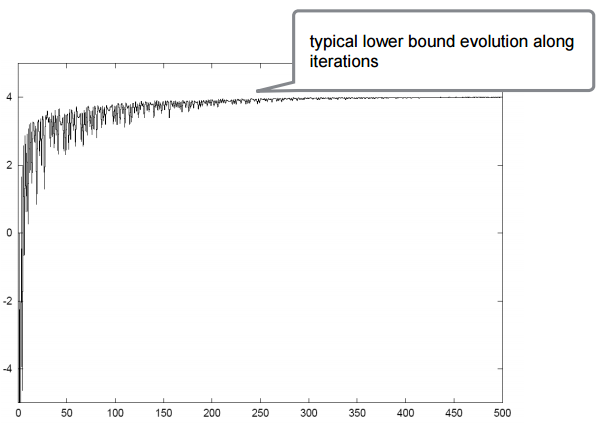
\includegraphics[scale=0.8]{lagrangeconverge.png}}



\section{Network flow}
%TODO slides 5



\section{Greedy and approximation algorithms}


\subsection{An activity-selection problem}
\begin{tabular}{m{6cm}m{10cm}}
    Find the max number of activities that do not
    overlap in time : 
    $$\forall i,j \quad selected: \quad s_i \geq f_j  \quad or \quad s_j \geq f_i$$
    &
\begin{itemize}
    \item $s_i$ = start time of activity
    \item $f_i$ = end time activity (not that activities are 
        sorted such that $f_i \leq f_{i+1}$)
\end{itemize}
\end{tabular}

\begin{enumerate}
    \item \textbf{Reduction} to the maximum independent set problem where 
        we find the maximum set of vertices in a graph such that
        to vertices selected are not adjacent.

        \begin{tabular}{m{10cm}m{3cm}}
            \begin{itemize}
                \item The reduction is done by add an edge between $i$ and $j$ if
                    activities overlap in time: 
                    $$s_i < f_j and s_j < f_i$$ 
            \end{itemize}
            Note that the maximum independent set problem is NP-Hard problem
            &
            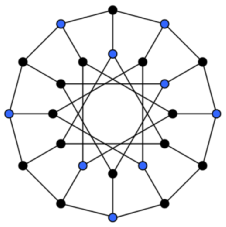
\includegraphics[width=3cm]{img/independant}
        \end{tabular}


    \item \textbf{Dynamic programming}: select a maximum size subset of mutually
        compatible activities from $S_{ij}$, for $0 \leq i < j \leq n+1$,
        knowing that all other $S_{ij}$ are empty.

        $a_m$ such that $f_m = min\{f_k: a_k \in S_{ij}\}$
        \[
            c[i, j] = 
            \begin{cases} 
                0 & \text{if } S_{ij} = \emptyset \\
                max_{\substack{i<k<j \\ a_k \in S_{ij}}} \{c[i, k] + c[k, j] + 1\}  & \text{if } S_{ij} \neq \emptyset
            \end{cases}
        \]
        \begin{itemize}
                %TODO
            \item Time complexity: 
            \item Space complexity: 
        \end{itemize}

        \paragraph{Improvement to a greedy}
        \begin{itemize}
            \item Obs.1: a m is used in some maximum-size subset of
                mutually compatible activities of $S_ij$

                Proof (Sketch):
                \begin{small}
                    Suppose $A_{ij}$ an optimal set of $S_{ij}$ . Take
                    the first activity of $A_{ij}$ (assume it is $a_k$ with $k \neq m$). We
                    can safely replace $a_k$ with $a_m$ because $f_m \leq f_k$.
                \end{small}

            \item Obs.2: The subproblem $S_im$ is empty, so that choosing
                $a_m$ (in the recurrence) leaves the subproblem $S_mj$ as the
                only one that may be nonempty.
        \end{itemize}

        %TODO new recurrence equation

    \item \textbf{Greedy algorithm}
        \begin{lstlisting}[mathescape]
n $=$ nbrActivities
A $= a_1$
i $= 1$

for m $\leftarrow$ 2 to n do
if $s_m \geq f_i$ then
A = $A \cup a_m$
i =$m$

return A
        \end{lstlisting}
\end{enumerate}


\subsection{Greedy}
At each decision point, the algorithm makes
a \textbf{local optimum choice} in the hope that it is a global
optimum choice.
\begin{itemize}
    \item For some problem it's the case
    \item For other it's not and sometimes we can 
        have a guarantee how
        \textit{suboptimal} we can be.
\end{itemize}


\subsection{Minimum Spanning Tree (MST)}

\subsubsection{Definition}
\begin{itemize}
    \item A \textbf{cut} (S,V-S) of an undirected graph
    \item An edge (u,v) \textbf{cross} the cut (S,V-S) if one of its
        endpoints is in S and the other in V-S
    \item A cut \textbf{respects} a set A of edges if no edge in A crosses
        the cut.
    \item An edge is a \textbf{light edge} crossing a cut if its weight is
        the minimum of any edge crossing the cut. (can be
        more than one in case of ties).
\end{itemize}

\subsubsection{Theorem}
\begin{itemize}
    \item[LET]
    \item $G=(V,E)$ a undirected graph with weight function $w$ on $E$.
    \item $A \subseteq E$ included in some MST for $G$.
    \item $(S, V-S)$ be any cut of $G$ that respect $A$
    \item $(u,v)$ be a light edge crossing $(S, V-S)$
    \item[THEN]
    \item edge $(u, v)$ is safe for $A$
    \end{itemize}

\subsubsection{Algorithm}

\begin{lstlisting}[mathescape, caption=Generic-MST(V\,E\,c\,s\,t)]
A = $\emptyset$
while A does not form a spanning tree do
    find an edge $(u, v)$ that is safe for A
    A = A $\cup \{(u, v)\}$

return A
\end{lstlisting}

\begin{itemize}
    \item \textbf{Kruskal} 

    \item \textbf{Prim} 
\end{itemize}

\subsection{Exam}
\begin{itemize}
    \item All theoretical notions introduced (proofs, etc).
    \item Design a greedy algorithm
    \item MST: I give you a new MST greedy algorithm. You
        should be able argument whether it is correct or not.
    \item Design a simple approximation scheme, compute it’s
        approximation ratio
    \item I give you a complexity of an approximation scheme.
        You should be able to tel me if it is fully polynomial.
\end{itemize}



\section{Local search}
%TODO slides 7


\section{Constraint programming}
%TODO slides 8


\section{Local Neighbors Search}
%TODO slides 9


\section{Derivative free optimization}
%TODO slides 10


\section{Bi-objective}
%TODO slides 11




\end{document}
